\documentclass[11pt,oneside]{article}

\usepackage[a4paper,margin=27mm,headheight=15pt]{geometry}
\usepackage[T1]{fontenc}
\usepackage[utf8]{inputenc}
\IfFileExists{libertinus.sty}{\usepackage{libertinus}}{\usepackage{lmodern}}
\usepackage{microtype}
\usepackage{amsmath,amssymb,amsthm,mathtools,mathrsfs}
\usepackage{bm}
\usepackage{booktabs,longtable,array,tabularx}
\usepackage{graphicx}
\usepackage{pgfplots}
\usepackage{xcolor}
\usepackage{enumitem}
\usepackage{fancyhdr}
\usepackage{titlesec}
\usepackage{listings}
\usepackage{xurl}
\usepackage{hyperref}
\usepackage[nameinlink,noabbrev]{cleveref}

\definecolor{linkblue}{RGB}{25,75,135}
\definecolor{shadegray}{RGB}{246,247,249}
\definecolor{rulegray}{RGB}{195,201,208}
\pgfplotsset{compat=1.18}
\hypersetup{
  colorlinks=true,
  linkcolor=linkblue,
  citecolor=linkblue,
  urlcolor=linkblue,
  pdftitle={Decay of the Fourier Transform of Rvachev's Up-Function},
  pdfsubject={Dyadic renormalization, transfer-operator norms, sharp envelopes, and exceptional valleys},
  pdfkeywords={Rvachev up-function, Fabius function, sinc product, Fourier transform, Thue-Morse, transfer operator, asymptotic decay}
}

\pagestyle{fancy}
\fancyhf{}
\fancyhead[L]{\small Fourier decay of Rvachev's up-function}
\fancyhead[R]{\small\nouppercase{\leftmark}}
\fancyfoot[C]{\thepage}
% Canonical project-wide mathematical notation.
% Canonical mathematical notation for active FabiusFunction LaTeX documents.
%
% This file is intentionally a plain TeX input rather than a LaTeX package.
% Every standalone document loads it by an explicit path relative to that
% document's directory; included fragments inherit the definitions from their
% root document.  Keep this file independent of document layout and metadata.
%
% Contract:
%   * one command has one mathematical meaning throughout the active corpus;
%   * names encode semantic roles rather than a document-local choice of letter;
%   * visually similar but differently normalized objects have different print;
%   * every command below is defined normatively in the notation catalogue.
%
% The active corpus excludes docs/archive/.  Historical sources may retain
% their original notation only inside an explicitly labelled quotation.

\makeatletter
\@ifundefined{mathbb}{%
  \PackageError{fabius-notation}{The amssymb package must be loaded first}%
    {Load amsmath and amssymb before inputting fabius-notation.tex.}%
}{}
\@ifundefined{operatorname}{%
  \PackageError{fabius-notation}{The amsmath package must be loaded first}%
    {Load amsmath before inputting fabius-notation.tex.}%
}{}
\makeatother

% Version stamp used by the catalogue and by static audits.
\newcommand{\FabiusNotationVersion}{2026-08-31}

% Number systems.  NaturalNumbers is explicitly the nonnegative convention.
\newcommand{\NaturalNumbers}{\mathbb{N}_{0}}
\newcommand{\PositiveIntegers}{\mathbb{N}_{>0}}
\newcommand{\IntegerNumbers}{\mathbb{Z}}
\newcommand{\RationalNumbers}{\mathbb{Q}}
\newcommand{\RealNumbers}{\mathbb{R}}
\newcommand{\ComplexNumbers}{\mathbb{C}}
\newcommand{\ExtendedRealNumbers}{\overline{\mathbb{R}}}

% The three principal Fabius--Rvachev functions.  Subscripts are deliberate:
% a bare F and a calligraphic F have several unrelated uses in the corpus.
\newcommand{\FabiusBounded}{F_{\mathrm{bd}}}
\newcommand{\FabiusGlobal}{F_{\mathrm{gl}}}
\newcommand{\FabiusQuantile}{Q_{F}}
\newcommand{\FabiusClampedQuantile}{Q_{F,\mathrm{cl}}}
\newcommand{\RvachevUp}{\operatorname{up}}

% Constants, elementary operators, and delimiters.
\newcommand{\EulerE}{\mathrm{e}}
\newcommand{\ImaginaryUnit}{\mathrm{i}}
\newcommand{\Differential}{\mathop{}\!\mathrm{d}}
\newcommand{\AbsoluteValue}[1]{\left\lvert #1\right\rvert}
\newcommand{\Norm}[1]{\left\lVert #1\right\rVert}
\newcommand{\Floor}[1]{\left\lfloor #1\right\rfloor}
\newcommand{\Ceiling}[1]{\left\lceil #1\right\rceil}
\newcommand{\FractionalPart}[1]{\left\{#1\right\}}
\newcommand{\PositivePart}[1]{\left(#1\right)_{+}}
\newcommand{\IndicatorOf}[1]{\mathbf{1}_{#1}}
\newcommand{\SetOf}[1]{\left\{#1\right\}}
\newcommand{\InnerProduct}[1]{\left\langle #1\right\rangle}
\newcommand{\CardinalityOf}[1]{\left\lvert #1\right\rvert}
\newcommand{\DefinitionEquals}{\mathrel{\coloneqq}}
\newcommand{\Sign}{\operatorname{sgn}}
\newcommand{\IdentityOperator}{\operatorname{id}}
\newcommand{\SpanOperator}{\operatorname{span}}
\newcommand{\TraceOperator}{\operatorname{tr}}
\newcommand{\RankOperator}{\operatorname{rank}}
\newcommand{\DiagonalOperator}{\operatorname{diag}}
\newcommand{\ResidueOperator}{\operatorname*{Res}}
\newcommand{\LeastCommonMultiple}{\operatorname{lcm}}
\newcommand{\OrderOperator}{\operatorname{ord}}
\newcommand{\PrincipalLogarithm}{\operatorname{Log}}
\newcommand{\FallingFactorial}[2]{\left(#1\right)^{\underline{#2}}}
\newcommand{\RisingFactorial}[2]{\left(#1\right)^{\overline{#2}}}

% Support, topology, convolution, and metric notation.
\newcommand{\SupportOperator}{\operatorname{supp}}
\newcommand{\SupportOf}[1]{\SupportOperator\!\left(#1\right)}
\newcommand{\TopologicalSupportOf}[1]{\operatorname{tsupp}\!\left(#1\right)}
\newcommand{\Convolution}{\mathbin{*}}
\newcommand{\MetricDistance}{\operatorname{dist}}
\newcommand{\TotalVariationDistance}{d_{\mathrm{TV}}}

% Probability.  Equality and convergence in law are not metric distance.
\newcommand{\Probability}{\mathbb{P}}
\newcommand{\Expectation}{\mathbb{E}}
\newcommand{\Variance}{\operatorname{Var}}
\newcommand{\Covariance}{\operatorname{Cov}}
\newcommand{\LawOperator}{\operatorname{Law}}
\newcommand{\LawOf}[1]{\LawOperator\!\left(#1\right)}
\newcommand{\EqualInLaw}{\mathrel{\overset{\mathrm{law}}{=}}}
\newcommand{\ConvergesInLaw}{\mathrel{\xrightarrow{\mathrm{law}}}}

% Fourier and integral transforms.  The printed labels expose normalization.
% FourierTwoPi uses exp(-2*pi*i*x*xi); FourierAngular uses exp(-i*x*omega).
\newcommand{\FourierTwoPi}[1]{\widehat{#1}_{\,2\pi}}
\newcommand{\FourierAngular}[1]{\widehat{#1}_{\,\mathrm{ang}}}
\newcommand{\LaplaceTransformSymbol}{\mathcal{L}}
\newcommand{\MellinTransformSymbol}{\mathcal{M}}
\newcommand{\LaplaceTransformOf}[1]{\LaplaceTransformSymbol\!\left[#1\right]}
\newcommand{\MellinTransformOf}[1]{\MellinTransformSymbol\!\left[#1\right]}
\newcommand{\MomentGeneratingFunction}[1]{M_{#1}}
\newcommand{\CharacteristicFunction}[1]{\varphi_{#1}}

% The two standard sinc functions must never share one symbol.
\newcommand{\SincRad}{\operatorname{sinc}_{\mathrm{rad}}}
\newcommand{\SincPi}{\operatorname{sinc}_{\pi}}

% Binary arithmetic and Thue--Morse notation.
\newcommand{\BinaryDigitSum}{\operatorname{wt}_{2}}
\newcommand{\ThueMorseSignSymbol}{\varepsilon}
\newcommand{\ThueMorseSign}[1]{\varepsilon_{#1}}
\newcommand{\PadicValuation}[1]{\nu_{#1}}
\newcommand{\TwoAdicValuation}{\nu_{2}}

% q-series notation.  Every base is an explicit argument.
\newcommand{\QPochhammer}[3]{\left(#1;#2\right)_{#3}}
\newcommand{\GaussianBinomial}[3]{%
  \genfrac{[}{]}{0pt}{}{#1}{#2}_{#3}%
}
\newcommand{\QInteger}[2]{\left[#1\right]_{#2}}

% Named special functions.
\newcommand{\Polylogarithm}{\operatorname{Li}}
\newcommand{\LambertW}{W}
\newcommand{\GammaFunction}{\Gamma}
\newcommand{\RiemannZeta}{\zeta}

% Asymptotics.  BigO and LittleO are operator tokens for existing formula
% grammar; prefer the At forms so that the limiting regime is printed.
\newcommand{\BigO}{\mathcal{O}}
\newcommand{\LittleO}{o}
\newcommand{\BigOAt}[2]{\mathcal{O}_{#2}\!\left(#1\right)}
\newcommand{\LittleOAt}[2]{o_{#2}\!\left(#1\right)}

\renewcommand{\headrulewidth}{0.4pt}

\titleformat{\section}{\Large\bfseries}{\thesection}{0.7em}{}
\titleformat{\subsection}{\large\bfseries}{\thesubsection}{0.7em}{}
\titleformat{\subsubsection}{\normalsize\bfseries}{\thesubsubsection}{0.7em}{}
\setcounter{secnumdepth}{3}
\setcounter{tocdepth}{2}
\setlist[itemize]{leftmargin=2em,itemsep=0.25em,topsep=0.4em}
\setlist[enumerate]{leftmargin=2.3em,itemsep=0.25em,topsep=0.4em}
\setlength{\emergencystretch}{2em}

\newtheorem{theorem}{Theorem}[section]
\newtheorem{proposition}[theorem]{Proposition}
\newtheorem{lemma}[theorem]{Lemma}
\newtheorem{corollary}[theorem]{Corollary}
\newtheorem{conjecture}[theorem]{Conjecture}
\theoremstyle{definition}
\newtheorem{definition}[theorem]{Definition}
\newtheorem{example}[theorem]{Example}
\theoremstyle{remark}
\newtheorem{remark}[theorem]{Remark}
\newtheorem{warning}[theorem]{Warning}

\newcommand{\Phiup}{\Phi}
\newcommand{\spec}{\operatorname{spr}}
\newcommand{\esssup}{\operatorname*{ess\,sup}}

\newenvironment{proofidea}{\par\smallskip\noindent\textit{Proof architecture.}\ }{\hfill$\square$\par\smallskip}
\newenvironment{boxedremark}{%
  \par\smallskip\noindent\begin{center}\begin{minipage}{0.94\textwidth}%
  \color{black}\hrule\vspace{0.6em}\small
}{%
  \vspace{0.6em}\hrule\end{minipage}\end{center}\smallskip
}

\lstdefinestyle{code}{
  basicstyle=\ttfamily\footnotesize,
  backgroundcolor=\color{shadegray},
  frame=single,
  rulecolor=\color{rulegray},
  columns=fullflexible,
  keepspaces=true,
  showstringspaces=false,
  breaklines=true,
  xleftmargin=0.7em,
  xrightmargin=0.7em,
  aboveskip=0.8em,
  belowskip=0.8em
}

\title{\bfseries Decay of the Fourier Transform of Rvachev's Up-Function\\[0.35em]
\large Dyadic renormalization, transfer-operator norms, sharp envelopes, and exceptional valleys}
\author{Research note for Vladimir Reshetnikov's \texttt{ProveIt} project}
\date{26 August 2026}

\begin{document}
\maketitle

\begin{abstract}
Let
\[
 \Phiup(x)=\widehat{\RvachevUp}(x)
 =\prod_{h=0}^{\infty}\SincRad\!\left(\frac{\pi x}{2^h}\right),
 \qquad \SincRad t=\frac{\sin t}{t},
\]
be the Fourier transform of Rvachev's compactly supported up-function.  The phrase
``the decay rate of $\Phiup$'' is intrinsically ambiguous: the function vanishes at every
nonzero integer, its values are controlled by a lacunary sine product, and even its local
extrema have exceptional deep valleys.  Consequently there is no global pointwise
asymptotic and no single log-normal--power envelope that makes all oscillations approach
one nonzero amplitude.

The exact dyadic factorization
\[
 \AbsoluteValue{\Phiup(2^n y)}
 =\AbsoluteValue{\Phiup(y)}\,\pi^{-n}y^{-n}2^{-n(n+1)/2}
   \prod_{j=1}^{n}\AbsoluteValue{\sin(\pi 2^j y)},
 \qquad \tfrac12\le y\le1,
\]
reduces every natural averaged notion of decay to a weighted doubling-map problem.  We
introduce a complete $L^q$ dyadic-shell spectrum.  With
\[
 E_\kappa(x)=\exp\!\left(-\frac{(\log x)^2}{2\log2}-\kappa\log x\right),
\]
the sharp exponents are
\[
\begin{array}{c|c}
\text{notion of amplitude}&\kappa\\ \hline
\text{geometric mean / almost-everywhere dyadic ray}
 &\displaystyle \frac32+\frac{\log\pi}{\log2}=3.151496129\ldots\\[0.4em]
\text{arithmetic mean of }\AbsoluteValue{\Phiup}
 &\displaystyle 2.748070014\ldots\\[0.3em]
\text{root mean square}
 &\displaystyle \frac{\log(2\pi)}{\log2}=2.651496129\ldots\\[0.5em]
\text{uniform upper envelope}
 &\displaystyle \frac32+\frac{\log(\pi/\sqrt3)}{\log2}
   =2.359014879\ldots .
\end{array}
\]
The arithmetic-mean constant is characterized rigorously by the Perron root of an explicit
transfer operator and is computed numerically to high precision.  The RMS exponent is
exact by Parseval, while the uniform exponent follows from an elementary sharp inequality
for lacunary sine products; equality is realized by the period-two orbit
$1/3\leftrightarrow2/3$.

We also prove: (i) every interval between consecutive integer zeros contains exactly one
extremum, whose sign is the signed Thue--Morse value; (ii) the normalized arithmetic means
have a nonconstant dyadic phase profile, so a plain Cesaro limit does not exist although the
weaker two-sided boundedness criterion does hold; and (iii) for each fixed $r\ge0$, the
extremum immediately to the right of $2^{n-1}+r$ satisfies an explicit asymptotic of order
$\exp(- (\log x)^2/\log2+\BigO(\log x))$, twice the generic log-square rate in the leading
quadratic term.  These results identify precisely what is correct in the existing decay-rate
draft: its power $x^{-\log(2\pi)/\log2}$ is the RMS power, not a pointwise or optimal-envelope
power, and no additional universal power of $\log x$ repairs that mismatch.
\end{abstract}

\tableofcontents
\newpage

\section{The question and the shape of the answer}
\label{sec:introduction}

Rvachev's up-function is the even $C^\infty$ probability density supported on $[-1,1]$
that is closely related to the Fabius distribution function.  Under the Fourier convention
\[
 \widehat f(\xi)=\int_{\RealNumbers}f(t)\EulerE^{-2\pi\ImaginaryUnit t\xi}\Differential t,
\]
its transform is the entire function
\begin{equation}
 \Phiup(z)=\widehat{\RvachevUp}(z)
 =\prod_{h=0}^{\infty}\SincRad\!\left(\frac{\pi z}{2^h}\right).
 \label{eq:Phi-definition}
\end{equation}
This formula is classical; see, for example, Arias de Reyna's systematic treatment
\cite{arias1982} and the Fabius/Rvachev development in \cite{proveit}.

The motivating questions in \cite{mse-extrema,mse-decay} ask for the amplitude of the
oscillations and, more specifically, for a positive elementary function $g$ such that an
average of $\AbsoluteValue{\Phiup}/g$ tends to one or at least stays between two positive constants.
A working draft in the \texttt{ProveIt} repository \cite{decay-draft} proposes a log-normal
factor together with the power $x^{-\log(2\pi)/\log2}$ and a possible power of $\log x$.
The log-normal factor is indeed fundamental, but the rest of the conclusion depends on
which norm or averaging operation is intended.

There are three separate obstructions to a single pointwise answer.

\begin{enumerate}
\item The transform has a zero at every nonzero integer, so no asymptotic
      $\AbsoluteValue{\Phiup(x)}\sim g(x)>0$ can hold on the full real ray.
\item After the deterministic denominator is removed, what remains is a Birkhoff product
      for the doubling map.  Its geometric mean, arithmetic mean, quadratic mean, and
      supremum have different exponential growth rates.
\item Even the unique maxima between consecutive zeros possess exceptional subsequences.
      The peaks associated with the binary period-two orbit attain the sharp global upper
      envelope, whereas the extrema in the first few intervals after a power of two are
      exponentially smaller on the $n^2$ scale.
\end{enumerate}

Thus the correct answer is a \emph{spectrum of decay rates}, not one formula.  A convenient
common scale is
\begin{equation}
 E_\kappa(x)
 :=\exp\!\left(-\frac{(\log x)^2}{2a}-\kappa\log x\right)
 =x^{-\kappa}\exp\!\left(-\frac{(\log x)^2}{2\log2}\right),
 \qquad a:=\log2.
 \label{eq:E-kappa}
\end{equation}
For fixed dyadic phase, the quadratic term in \eqref{eq:E-kappa} comes from the product of
the $n$ denominators $2^1,\dots,2^n$.  The linear term is where the lacunary numerator
enters.

\subsection{Main decay table}
\label{subsec:main-table}

The following table summarizes the results proved below.  In the finite-$q$ rows,
``normalized'' means the normalized $L^q$ norm on the dyadic shell
$[2^{n-1},2^n]$.

\begin{center}
\begin{tabularx}{\textwidth}{@{}>{\raggedright\arraybackslash}p{0.24\textwidth}
  >{\centering\arraybackslash}p{0.20\textwidth}
  >{\centering\arraybackslash}p{0.25\textwidth}
  X@{}}
\toprule
Amplitude notion & numerator scale $\Lambda$ & power $\kappa$ in $E_\kappa$ & conclusion\\
\midrule
Geometric mean ($q=0$) and typical dyadic ray
 & $1/2$
 & $\displaystyle \frac32+\frac{\log\pi}{a}$
 & shell geometric mean is exactly constant after normalization; the same exponent holds
   for Lebesgue-a.e. fixed phase\\[0.7em]
Arithmetic mean ($q=1$)
 & $\rho_1=0.6613226021\ldots$
 & $\displaystyle \frac{\log\pi+a/2-\log\rho_1}{a}$
 & shell means converge to a positive constant; ordinary Cesaro means have a nonconstant
   dyadic phase profile\\[0.7em]
Root mean square ($q=2$)
 & $2^{-1/2}$
 & $\displaystyle \frac{\log(2\pi)}{a}$
 & exact numerator identity $\int B_n^2=2^{-n}$; normalized shell RMS converges\\[0.7em]
Uniform envelope ($q=\infty$)
 & $\sqrt3/2$
 & $\displaystyle \frac32+\frac{\log(\pi/\sqrt3)}{a}$
 & global upper bound, sharp on $x=2^n(2/3)$; not a two-sided envelope for every extremum\\
\bottomrule
\end{tabularx}
\end{center}

The ordering is
\begin{equation}
 \begin{aligned}
 \kappa_\infty&=2.359014879\ldots<\kappa_2=2.651496129\ldots\\
 &<\kappa_1=2.748070014\ldots<\kappa_0=3.151496129\ldots .
 \end{aligned}
 \label{eq:kappa-order}
\end{equation}
Larger $q$ emphasizes rarer and larger values, hence gives a slower decay and a smaller
power $\kappa_q$.

\begin{boxedremark}
The coefficient $\log(2\pi)/\log2$ appearing in the working draft is not an accidental
near miss.  It is \emph{exactly} the root-mean-square power $\kappa_2$.  It is not the
arithmetic-mean power, the typical power, or the sharp uniform-envelope power.  No factor
$(\log x)^p$ can convert one of these powers into another, because their discrepancy is
already a nonzero multiple of $\log x$ in the logarithm of the amplitude.
\end{boxedremark}

\section{Exact products, zeros, and scaling laws}
\label{sec:exact-products}

\subsection{Entire convergence and three product forms}

The compact convergence of \eqref{eq:Phi-definition} follows from
\[
 \SincRad w=1-\frac{w^2}{6}+\BigO(w^4),
 \qquad
 \sum_{h\ge0}\frac{\AbsoluteValue z^2}{4^h}<\infty
\]
uniformly for $z$ in a compact set.  Hence $\Phiup$ is even, real on $\RealNumbers$, entire, and
$\Phiup(0)=1$.

Vieta's product $\SincRad t=\prod_{j\ge1}\cos(t/2^j)$ and Euler's sine product give two other
useful forms:
\begin{equation}
 \Phiup(z)
 =\prod_{j=1}^{\infty}\cos^j\!\left(\frac{\pi z}{2^j}\right)
 =\prod_{m=1}^{\infty}
   \left(1-\frac{z^2}{m^2}\right)^{1+\TwoAdicValuation(m)}.
 \label{eq:three-products}
\end{equation}
Indeed, in the cosine product the factor with denominator $2^j$ occurs for exactly $j$
pairs of indices.  In the Weierstrass product, the integer $m$ is a zero of the sinc factor
at level $h$ precisely when $2^h\mid m$, so its total multiplicity is $1+\TwoAdicValuation(m)$.

The elementary one-step scaling law is
\begin{equation}
 \Phiup(2x)=\SincRad(2\pi x)\Phiup(x),
 \qquad
 \Phiup(x)=\SincRad(\pi x)\Phiup(x/2).
 \label{eq:one-step-scaling}
\end{equation}

\subsection{Zeros and their multiplicities}

\begin{proposition}[Integer zero divisor]
\label{prop:zero-divisor}
The nonzero zeros of $\Phiup$ are exactly the nonzero integers.  The zero at
$m\in\IntegerNumbers\setminus\{0\}$ has multiplicity
\[
 d(m)=1+\TwoAdicValuation(\AbsoluteValue m).
\]
Moreover, if $b\ge1$ is an integer, $d=1+\TwoAdicValuation(b)$, and $z\uparrow b$, then
\begin{equation}
 \AbsoluteValue{\Phiup(z)}
 =b^{-d}\AbsoluteValue{\Phiup(b/2^d)}(b-z)^d\bigl(1+\BigO(b-z)\bigr).
 \label{eq:zero-local-coefficient}
\end{equation}
\end{proposition}

\begin{proof}
The divisor statement follows immediately from the last product in
\eqref{eq:three-products}.  For the local coefficient, the vanishing factors are those with
$0\le h\le\TwoAdicValuation(b)$.  At $z=b$ each has a simple zero and
\[
 \AbsoluteValue{\frac{\Differential}{\Differential z}\SincRad\!\left(\frac{\pi z}{2^h}\right)\Big|_{z=b}}
 =\frac1b.
\]
The product of the remaining factors is
\[
 \prod_{h=d}^{\infty}
 \AbsoluteValue{\SincRad\!\left(\frac{\pi b}{2^h}\right)}
 =\AbsoluteValue{\Phiup(b/2^d)}.
\]
Multiplication gives \eqref{eq:zero-local-coefficient}.
\end{proof}

\subsection{Exact dyadic renormalization}
\label{subsec:dyadic-renormalization}

Let
\[
 T(x)=2x\pmod1,
 \qquad
 s(x)=\AbsoluteValue{\sin(\pi x)},
 \qquad x\in[0,1],
\]
and define the lacunary product
\begin{equation}
 B_n(y):=\prod_{j=1}^{n}s(T^j y)
 =\prod_{j=1}^{n}\AbsoluteValue{\sin(\pi2^j y)}.
 \label{eq:Bny}
\end{equation}

\begin{theorem}[Exact dyadic factorization]
\label{thm:exact-dyadic-factorization}
For every $n\ge1$ and $y\in[1/2,1]$,
\begin{equation}
 \AbsoluteValue{\Phiup(2^n y)}
 =\AbsoluteValue{\Phiup(y)}\,\pi^{-n}y^{-n}2^{-n(n+1)/2}B_n(y).
 \label{eq:exact-factorization}
\end{equation}
For any real $\kappa$, set
\begin{equation}
 W_\kappa(y)
 :=\AbsoluteValue{\Phiup(y)}y^\kappa
   \exp\!\left(\frac{(\log y)^2}{2a}\right).
 \label{eq:W-kappa}
\end{equation}
Then the following normalized identity is exact:
\begin{equation}
 \frac{\AbsoluteValue{\Phiup(2^n y)}}{E_\kappa(2^n y)}
 =W_\kappa(y)
  \exp\!\left(n(\kappa a-\log\pi-a/2)\right)B_n(y).
 \label{eq:master-normalization}
\end{equation}
\end{theorem}

\begin{proof}
Iterating \eqref{eq:one-step-scaling} gives
\[
 \Phiup(2^n y)=\Phiup(y)\prod_{j=1}^{n}\SincRad(\pi2^j y).
\]
The product of the denominators is
$\pi^ny^n2^{1+\cdots+n}=\pi^ny^n2^{n(n+1)/2}$, proving
\eqref{eq:exact-factorization}.  Write $L=\log(2^ny)=na+\log y$ and divide
\eqref{eq:exact-factorization} by
$\exp(-L^2/(2a)-\kappa L)$.  The terms $-n\log y$ cancel, leaving
\eqref{eq:master-normalization}.
\end{proof}

Equation \eqref{eq:master-normalization} is the central identity of this article.  The
entire deterministic decay has been extracted into $E_\kappa$.  The bounded phase factor
$W_\kappa$ and the dynamical product $B_n$ contain all remaining information.

\subsection{The Thue--Morse polynomial}

Let $\tau_k=(-1)^{s_2(k)}$, where $s_2(k)$ is the number of ones in the binary expansion of
$k$.  The finite product identity
\begin{equation}
 P_n(x):=\prod_{j=0}^{n-1}(1-\EulerE^{2\pi\ImaginaryUnit2^jx})
 =\sum_{k=0}^{2^n-1}\tau_k\EulerE^{2\pi\ImaginaryUnit kx}
 \label{eq:TM-polynomial}
\end{equation}
follows by induction.  Taking moduli yields
\begin{equation}
 \AbsoluteValue{P_n(x)}=2^n\prod_{j=0}^{n-1}s(T^jx).
 \label{eq:TM-modulus}
\end{equation}
Thus the same products governing the decay of $\widehat{\RvachevUp}$ are the normalized moduli of
classical Thue--Morse trigonometric polynomials.  This is the bridge to Gelfond exponents,
Riesz products, and thermodynamic formalism; see \cite{gelfond,queffelec,fan-schmeling-shen}.

\subsection{A second exact scaling identity}
\label{subsec:boundary-identity}

The behavior just to the right of a large dyadic integer is exposed by a different exact
identity.

\begin{lemma}[Dyadic-boundary identity]
\label{lem:dyadic-boundary}
Let $N=2^{n-1}$ and $0<z<N$.  Then
\begin{equation}
 \AbsoluteValue{\Phiup(N+z)}
 =\frac{\AbsoluteValue{\Phiup(\tfrac12+z/(2N))}}
        {\AbsoluteValue{\Phiup(z/(2N))}}
  \left(\frac{z}{N+z}\right)^n\AbsoluteValue{\Phiup(z)}.
 \label{eq:dyadic-boundary}
\end{equation}
\end{lemma}

\begin{proof}
For $0\le h<n$, the number $N/2^h$ is an integer, so
\[
 \AbsoluteValue{\sin(\pi(N+z)/2^h)}=\AbsoluteValue{\sin(\pi z/2^h)}.
\]
The quotient of the first $n$ sinc factors is therefore $(z/(N+z))^n$ in absolute value.
Reindexing the remaining tails gives
\[
 \prod_{h=n}^{\infty}\SincRad\!\left(\frac{\pi(N+z)}{2^h}\right)
 =\Phiup\!\left(\frac12+\frac{z}{2N}\right),
 \quad
 \prod_{h=n}^{\infty}\SincRad\!\left(\frac{\pi z}{2^h}\right)
 =\Phiup\!\left(\frac{z}{2N}\right).
\]
Combining the finite and infinite parts proves the identity.
\end{proof}

\section{Exactly one extremum per unit interval}
\label{sec:extrema}

The Weierstrass product gives a short complete proof of the observed one-extremum property.

\begin{theorem}[Strict logarithmic concavity between zeros]
\label{thm:unique-extremum}
The function $\Phiup$ is positive and strictly decreasing on $(0,1)$.  For every integer
$m\ge1$, $\AbsoluteValue{\Phiup}$ has exactly one critical point
$\xi_m\in(m,m+1)$.  It is the strict maximum of $\AbsoluteValue{\Phiup}$ on that interval.  Moreover,
for every integer $m\ge0$,
\begin{equation}
 \Sign\Phiup(x)=(-1)^{s_2(m)},\qquad m<x<m+1.
 \label{eq:TM-sign}
\end{equation}
For $m\ge1$ the signed extremum is therefore
$\Phiup(\xi_m)=(-1)^{s_2(m)}M_m$, where
\[
 M_m:=\max_{m\le x\le m+1}\AbsoluteValue{\Phiup(x)}.
\]
\end{theorem}

\begin{proof}
Away from the integer zeros, termwise logarithmic differentiation of
\eqref{eq:three-products} is locally uniform and gives
\begin{align}
 \frac{\Differential}{\Differential x}\log\AbsoluteValue{\Phiup(x)}
 &=-2x\sum_{k=1}^{\infty}\frac{1+\TwoAdicValuation(k)}{k^2-x^2},
 \label{eq:log-derivative}\\
 \frac{\Differential^2}{\Differential x^2}\log\AbsoluteValue{\Phiup(x)}
 &=-2\sum_{k=1}^{\infty}(1+\TwoAdicValuation(k))
   \frac{k^2+x^2}{(k^2-x^2)^2}<0.
 \label{eq:strict-log-concavity}
\end{align}
For $0<x<1$, every denominator in \eqref{eq:log-derivative} is positive, so
$(\log\Phiup)'(x)<0$.  This proves strict decrease on the first interval.

Now let $m\ge1$.  The logarithmic derivative is strictly decreasing on $(m,m+1)$.
The pole contributed by $k=m$ forces it to $+\infty$ at the left endpoint, while the pole
contributed by $k=m+1$ forces it to $-\infty$ at the right endpoint.  It therefore has
exactly one zero, and strict log-concavity makes that point the unique maximum of the modulus.

Starting from $\Phiup(0)=1$, crossing the zero at $k$ changes the sign
$1+\TwoAdicValuation(k)$ times.  Therefore the sign on $(m,m+1)$ is
\[
 (-1)^{\sum_{k=1}^{m}(1+\TwoAdicValuation(k))}.
\]
Legendre's identity $\TwoAdicValuation(m!)=m-s_2(m)$ gives
\[
 \sum_{k=1}^{m}(1+\TwoAdicValuation(k))=m+\TwoAdicValuation(m!)=2m-s_2(m),
\]
whose parity is $s_2(m)$.  This proves \eqref{eq:TM-sign}.
\end{proof}

\begin{remark}
The critical points do \emph{not} in general converge to the midpoints of their unit
intervals.  In \Cref{sec:exceptional-extrema} we prove that, in every fixed interval offset
from a large power of two, the critical point approaches the \emph{right} endpoint at rate
$1/n$.
\end{remark}

\section{Dyadic-shell means and the transfer operator}
\label{sec:Lq-spectrum}

\subsection{Normalized shell means}

For $q\in(0,\infty)$ and a measurable $H$ on the shell
$D_n=[2^{n-1},2^n]$, define
\begin{equation}
 \mathcal M_{q,n}(H)
 :=\left(\frac1{2^{n-1}}\int_{2^{n-1}}^{2^n}\AbsoluteValue{H(x)}^q\Differential x\right)^{1/q}
 =\left(2\int_{1/2}^{1}\AbsoluteValue{H(2^ny)}^q\Differential y\right)^{1/q}.
 \label{eq:shell-Lq}
\end{equation}
The endpoint conventions are
\begin{align}
 \mathcal M_{0,n}(H)
 &:=\exp\!\left(\frac1{2^{n-1}}
       \int_{2^{n-1}}^{2^n}\log\AbsoluteValue{H(x)}\Differential x\right),
 \label{eq:shell-L0}\\
 \mathcal M_{\infty,n}(H)
 &:=\sup_{2^{n-1}\le x\le2^n}\AbsoluteValue{H(x)}.
 \label{eq:shell-Linf}
\end{align}
The logarithm in \eqref{eq:shell-L0} is locally integrable despite the finitely many zeros.

After $y=(x+1)/2$, the numerator in \eqref{eq:master-normalization} becomes
\begin{equation}
 \prod_{j=0}^{n-1}s(T^jx),
 \qquad 0\le x\le1.
 \label{eq:forward-product}
\end{equation}
This product is generated by an explicit Perron--Frobenius operator.

\subsection{The weighted doubling operator}

For $q>0$, define
\begin{equation}
 (\mathcal L_q f)(x)
 :=\frac12\left[
   \sin^q\!\left(\frac{\pi x}{2}\right)f(x/2)
  +\cos^q\!\left(\frac{\pi x}{2}\right)f((x+1)/2)
 \right].
 \label{eq:transfer-operator}
\end{equation}
The factor $1/2$ makes this the Lebesgue Perron operator with weight $s^q$.
For every integrable $f$,
\begin{equation}
 \int_0^1 f(x)\prod_{j=0}^{n-1}s(T^jx)^q\Differential x
 =\int_0^1(\mathcal L_q^n f)(x)\Differential x.
 \label{eq:transfer-duality}
\end{equation}

We use the following standard Ruelle--Perron--Frobenius fact.  The weights in
\eqref{eq:transfer-operator} are nonnegative rather than strictly positive at the two
endpoints, but the two-branch system is primitive, so the usual cone and
Lasota--Yorke proof applies without alteration; see \cite[Chs.~2--3]{baladi} and the
singular-potential discussion in \cite{fan1997,fan-schmeling-shen}.

\begin{proposition}[Perron root and spectral decomposition]
\label{prop:RPF}
For every $q>0$, $\mathcal L_q$ has a simple leading eigenvalue
$\rho_q>0$, a strictly positive eigenfunction $h_q$, and a positive eigenmeasure $\nu_q$,
which may be normalized by
\[
 \mathcal L_qh_q=\rho_qh_q,
 \qquad
 \mathcal L_q^*\nu_q=\rho_q\nu_q,
 \qquad
 \nu_q(h_q)=1.
\]
On a suitable Holder space $C^\alpha[0,1]$, with
$0<\alpha\le\min(1,q)$, there is a spectral gap and
\begin{equation}
 \rho_q^{-n}\mathcal L_q^nf
 =\nu_q(f)h_q+\BigO(\vartheta_q^n\Norm f_{C^\alpha}),
 \qquad 0<\vartheta_q<1.
 \label{eq:RPF-convergence}
\end{equation}
The same conclusion applies to nonnegative endpoint-power functions encountered below by
choosing a compatible Holder exponent.
\end{proposition}

\subsection{The full finite-$q$ decay spectrum}

Set
\begin{equation}
 \Lambda_q:=\rho_q^{1/q},
 \qquad
 \kappa_q:=\frac{\log\pi+a/2-\log\Lambda_q}{a},
 \qquad q>0.
 \label{eq:kappa-q}
\end{equation}

\begin{theorem}[Sharp finite-$q$ shell asymptotics]
\label{thm:Lq-spectrum}
For every $q\in(0,\infty)$ there is a constant $A_q\in(0,\infty)$ such that
\begin{equation}
 \mathcal M_{q,n}\!\left(\frac{\Phiup}{E_{\kappa_q}}\right)
 \longrightarrow A_q
 \qquad(n\to\infty).
 \label{eq:Lq-limit}
\end{equation}
More explicitly, with
\[
 \widetilde W_{q}(x)
 :=W_{\kappa_q}\!\left(\frac{x+1}{2}\right)^q,
\]
and the normalization in \Cref{prop:RPF},
\begin{equation}
 A_q^q=\left(\int_0^1h_q(x)\Differential x\right)\nu_q(\widetilde W_q).
 \label{eq:Aq}
\end{equation}
The number $\Lambda_q$ is nondecreasing in $q$, and therefore $\kappa_q$ is nonincreasing.
\end{theorem}

\begin{proof}
Raise \eqref{eq:master-normalization} to the $q$th power, use
\eqref{eq:shell-Lq}, and substitute $x=2y-1$.  This gives
\begin{align*}
 \mathcal M_{q,n}\!\left(\frac{\Phiup}{E_\kappa}\right)^q
 &=\exp\!\left(qn(\kappa a-\log\pi-a/2)\right)\\
 &\quad\times\int_0^1
 W_\kappa\!\left(\frac{x+1}{2}\right)^q
 \prod_{j=0}^{n-1}s(T^jx)^q\Differential x.
\end{align*}
By \eqref{eq:transfer-duality} and \eqref{eq:RPF-convergence}, the integral equals
\[
 \rho_q^n\left(\int_0^1h_q\right)
 \nu_q\!\left(W_\kappa((\,\cdot\,+1)/2)^q\right)(1+o(1)).
\]
The definition \eqref{eq:kappa-q} is exactly the cancellation condition
\[
 q(\kappa_q a-\log\pi-a/2)+\log\rho_q=0.
\]
This proves \eqref{eq:Lq-limit} and \eqref{eq:Aq}.

For each $n$, the $L^q$ norm of the product \eqref{eq:forward-product} on the probability
space $[0,1]$ is nondecreasing in $q$.  Taking $n$th roots and then the limit proves that
$\Lambda_q$ is nondecreasing.  Formula \eqref{eq:kappa-q} then gives the opposite
monotonicity of $\kappa_q$.
\end{proof}

\begin{remark}[No logarithmic-power correction]
\label{rem:no-log-correction}
For a fixed $q\in(0,\infty)$, replacing $E_{\kappa_q}$ by
$E_{\kappa_q}(\log x)^p$ multiplies the normalized shell mean by
$(na)^{-p}(1+o(1))$.  It therefore tends to $0$ when $p>0$ and to $+\infty$ when $p<0$.
At the sharp power, the required logarithmic exponent is $p=0$.
\end{remark}

\section{Geometric-mean and typical decay}
\label{sec:typical}

The $q=0$ endpoint is especially simple because Lebesgue measure is invariant under the
doubling map and
\begin{equation}
 \int_0^1\log\sin(\pi x)\Differential x=-\log2=-a.
 \label{eq:log-sine-integral}
\end{equation}

\begin{theorem}[Exact shell geometric mean]
\label{thm:geometric-mean}
Define
\begin{equation}
 \kappa_0:=\frac32+\frac{\log\pi}{a}
 =3.151496129472319\ldots .
 \label{eq:kappa0}
\end{equation}
Then
\begin{equation}
 \mathcal M_{0,n}\!\left(\frac{\Phiup}{E_{\kappa_0}}\right)
 =\exp\!\left(\int_0^1
    \log W_{\kappa_0}\!\left(\frac{x+1}{2}\right)\Differential x\right)
 \label{eq:exact-geometric-mean}
\end{equation}
for every $n\ge1$.  In particular, the normalized shell geometric mean is not merely
asymptotically constant; it is exactly independent of the shell.
\end{theorem}

\begin{proof}
Take logarithms in \eqref{eq:master-normalization}, substitute $x=2y-1$, and average.
The $n$ logarithmic sine terms each have integral $-a$ by invariance and
\eqref{eq:log-sine-integral}.  For \eqref{eq:kappa0},
\[
 \kappa_0a-\log\pi-a/2=a,
\]
so the linear contribution $na$ cancels the integral $-na$ exactly.
\end{proof}

The same exponent governs almost every fixed dyadic phase.

\begin{corollary}[Almost-everywhere dyadic-ray decay]
\label{cor:typical-ray}
For Lebesgue-a.e. $y\in[1/2,1]$,
\begin{equation}
 \log\AbsoluteValue{\Phiup(2^ny)}
 =-\frac{(\log(2^ny))^2}{2a}
  -\kappa_0\log(2^ny)+o(n).
 \label{eq:typical-ray}
\end{equation}
Equivalently,
\[
 \AbsoluteValue{\Phiup(2^ny)}=E_{\kappa_0}(2^ny)\EulerE^{o(n)}.
\]
\end{corollary}

\begin{proof}
The function $\log s$ is integrable and the doubling map is ergodic.  Birkhoff's theorem
therefore gives
\[
 \frac1n\log B_n(y)=\frac1n\sum_{j=1}^{n}\log s(T^jy)\longrightarrow-a
\]
for almost every $y$.  Substitute this in \eqref{eq:master-normalization} with
$\kappa=\kappa_0$.
\end{proof}

The $o(n)$ in \eqref{eq:typical-ray} is genuinely dynamical; it need not converge to a
constant.  Thus even the ``typical'' statement is a logarithmic asymptotic, not a pointwise
equivalent with one universal prefactor.

\section{The exact RMS power}
\label{sec:RMS}

For $q=2$, the transfer operator simplifies dramatically:
\begin{equation}
 \mathcal L_2\mathbf1
 =\frac12\left(\sin^2\frac{\pi x}{2}+\cos^2\frac{\pi x}{2}\right)
 =\frac12\mathbf1.
 \label{eq:L2-one}
\end{equation}
Its operator norm on $C[0,1]$ is at most $1/2$, so
\begin{equation}
 \rho_2=\frac12,
 \qquad
 \Lambda_2=\frac1{\sqrt2}.
 \label{eq:rho2}
\end{equation}
There is also a completely finite Fourier proof.  Parseval applied to
\eqref{eq:TM-polynomial} gives
\[
 \int_0^1\AbsoluteValue{P_n(x)}^2\Differential x=2^n,
\]
while \eqref{eq:TM-modulus} gives
\begin{equation}
 \int_0^1\prod_{j=0}^{n-1}s(T^jx)^2\Differential x=2^{-n}.
 \label{eq:exact-L2-product}
\end{equation}

\begin{corollary}[RMS decay]
\label{cor:RMS-decay}
The sharp root-mean-square exponent is
\begin{equation}
 \boxed{\displaystyle
 \kappa_2=\frac{\log(2\pi)}{\log2}
 =2.651496129472318\ldots .}
 \label{eq:kappa2}
\end{equation}
There is a constant $A_2\in(0,\infty)$ such that
\begin{equation}
 \mathcal M_{2,n}\!\left(\frac{\Phiup}{E_{\kappa_2}}\right)
 \longrightarrow A_2.
 \label{eq:RMS-limit}
\end{equation}
No power of $\log x$ belongs in the leading RMS normalization.
\end{corollary}

\begin{remark}[What the draft computed]
The power $x^{-\log(2\pi)/\log2}$ in \cite{decay-draft} is precisely
$x^{-\kappa_2}$.  Thus the draft identified the quadratic-mean scale, albeit without
specifying that norm.  Its claimed pointwise equivalent and its proposed logarithmic
correction do not follow and are incompatible with the exact shell identity
\eqref{eq:exact-L2-product}, the integer zeros, and the exceptional extrema proved later.
\end{remark}

\section{Arithmetic-mean decay and the Cesaro question}
\label{sec:L1-Cesaro}

\subsection{The Perron root $\rho_1$}

For $q=1$,
\begin{equation}
 (\mathcal L_1f)(x)
 =\frac12\left[
  \sin\frac{\pi x}{2}\,f(x/2)
 +\cos\frac{\pi x}{2}\,f((x+1)/2)
 \right].
 \label{eq:L1}
\end{equation}
There appears to be no elementary closed form for its Perron root.  It is nevertheless an
exact, canonical constant, and it is easy to compute stably:
\begin{equation}
 \rho_1=0.661322602060565\ldots .
 \label{eq:rho1-numerical}
\end{equation}
The corresponding power is
\begin{equation}
 \boxed{\displaystyle
 \kappa_1
 =\frac{\log\pi+a/2-\log\rho_1}{a}
 =2.748070014871335\ldots .}
 \label{eq:kappa1}
\end{equation}

The decimal in \eqref{eq:rho1-numerical} is numerical, but the following elementary
Collatz--Wielandt certificate provides a rigorous enclosure.

\begin{proposition}[A rational enclosure for $\rho_1$]
\label{prop:rho1-rigorous-bound}
One has
\begin{equation}
 0.66126807<\rho_1<0.66134891,
 \label{eq:rho1-rigorous-bound}
\end{equation}
and consequently
\begin{equation}
 2.74801262<\kappa_1<2.74818899.
 \label{eq:kappa1-rigorous-bound}
\end{equation}
\end{proposition}

\begin{proof}
For a positive continuous test function $f$, the Collatz--Wielandt inequalities give
\[
 \inf_{x\in[0,1]}\frac{\mathcal L_1f(x)}{f(x)}
 \le\rho_1\le
 \sup_{x\in[0,1]}\frac{\mathcal L_1f(x)}{f(x)}.
\]
Take
\[
 f(x)=F(\sin\pi x),\qquad
 F(u)=1+\frac{376189}{10^6}u-\frac{69093}{10^6}u^2
       +\frac{15483}{10^6}u^3.
\]
This function is positive on $[0,1]$.  Put $t=\tan(\pi x/4)\in[0,1]$,
$u=2t/(1+t^2)$, and $v=(1-t^2)/(1+t^2)$.  Then
\[
 \frac{\mathcal L_1f(x)}{f(x)}
 =\frac{uF(u)+vF(v)}{2F(2uv)},
\]
a rational function of $t$.  Exact Sturm-sequence checks show that the numerators of its
differences from the two rational endpoints in \eqref{eq:rho1-rigorous-bound} are positive
and have no zeros on $[0,1]$.  A compact exact-arithmetic verification is included in
\Cref{app:certificate}.
\end{proof}

\subsection{Sharp dyadic-shell mean}

By \Cref{thm:Lq-spectrum}, there is $A_1>0$ such that
\begin{equation}
 2\int_{1/2}^{1}
 \frac{\AbsoluteValue{\Phiup(2^ny)}}{E_{\kappa_1}(2^ny)}\Differential y
 \longrightarrow A_1.
 \label{eq:L1-shell-mean}
\end{equation}
Therefore the choice
\begin{equation}
 g_1(x):=A_1E_{\kappa_1}(x)
 \label{eq:g1}
\end{equation}
makes the mean of $\AbsoluteValue{\Phiup}/g_1$ on each dyadic shell tend to one.  This gives the
precise answer to the natural shell version of the question in \cite{mse-decay}.

It also answers the weaker full-ray boundedness question.

\begin{corollary}[Two-sided Cesaro boundedness]
\label{cor:Cesaro-boundedness}
For every fixed $t_0>0$, there are constants $0<c<C<\infty$ such that, for all sufficiently
large $t$,
\begin{equation}
 c<\frac1{t-t_0}\int_{t_0}^{t}
 \frac{\AbsoluteValue{\Phiup(x)}}{E_{\kappa_1}(x)}\Differential x<C.
 \label{eq:Cesaro-boundedness}
\end{equation}
After multiplying $E_{\kappa_1}$ by $A_1$, the same average tends to one along the dyadic
endpoints $t=2^n$.
\end{corollary}

\begin{proof}
Equation \eqref{eq:L1-shell-mean} says that the integral over the shell
$[2^{n-1},2^n]$ is asymptotic to $A_1 2^{n-1}$.  Summing the geometric sequence of completed
shells proves the dyadic-endpoint limit.  If $t$ lies inside the next shell, the completed
shells already contribute a positive constant times $t$, while the entire current shell
contributes at most another constant times $t$.  This gives \eqref{eq:Cesaro-boundedness}.
\end{proof}

\subsection{Why the ordinary Cesaro limit has a dyadic phase}
\label{subsec:phase-profile}

The full limit in the stronger condition of \cite{mse-decay} does not follow from the shell
limit.  In fact, the natural normalization \eqref{eq:g1} has a nonconstant phase profile.
This can be stated exactly in terms of the eigenmeasure of $\mathcal L_1$.

Normalize $h_1,\nu_1$ as in \Cref{prop:RPF}, and put
\[
 f_1(x):=W_{\kappa_1}\!\left(\frac{x+1}{2}\right),
 \qquad
 \mathscr F(z):=
 \frac{\nu_1(f_1\mathbf1_{[0,z]})}{\nu_1(f_1)},
 \quad 0\le z\le1.
 \label{eq:phase-distribution}
\]
The measure $f_1\,\Differential\nu_1$ is non-atomic, so $\mathscr F$ is continuous.  Here is a
short verification.  The endpoint atoms of $\nu_1$ vanish because the corresponding
transfer weights vanish.  For $z\in(0,1)\setminus\{1/2\}$, the eigenmeasure equation gives
\[
 \rho_1\nu_1(\{z\})=\frac12s(z)\nu_1(\{Tz\}).
\]
(The possible atom at $1/2$ is fed only by the already vanishing endpoint atoms.)  Hence any
remaining atom would generate forward atoms whose masses grow by at least the factor
$2\rho_1>1$ at every step.  A periodic orbit gives an immediate contradiction, and a
nonperiodic orbit would produce masses exceeding the finite total mass.  Thus $\nu_1$, and
therefore $f_1\,\Differential\nu_1$, has no atoms.

\begin{theorem}[Dyadic phase limit]
\label{thm:phase-limit}
For every $y\in[1/2,1]$ and every fixed $t_0>0$,
\begin{equation}
 \lim_{n\to\infty}
 \frac1{2^ny-t_0}\int_{t_0}^{2^ny}
 \frac{\AbsoluteValue{\Phiup(x)}}{A_1E_{\kappa_1}(x)}\Differential x
 =\mathscr P(y):=\frac{1+\mathscr F(2y-1)}{2y}.
 \label{eq:phase-limit}
\end{equation}
The continuous function $\mathscr P$ satisfies
$\mathscr P(1/2)=\mathscr P(1)=1$ but is not identically one.  Consequently the ordinary
Cesaro limit for the natural elementary scale $A_1E_{\kappa_1}$ does not exist.
\end{theorem}

\begin{proof}
The spectral decomposition gives, for $z\in[0,1]$,
\[
 \rho_1^{-n}\int_0^z f_1(x)
 \prod_{j=0}^{n-1}s(T^jx)\Differential x
 \longrightarrow
 \left(\int_0^1h_1\right)\nu_1(f_1\mathbf1_{[0,z]}).
\]
Approximation from above and below by Holder functions justifies the indicator; the
leading conformal measure has no atoms.  Returning to the shell variable, the partial
integral from $2^{n-1}$ to $2^ny$ is asymptotic to
\[
 2^{n-1}A_1\mathscr F(2y-1).
\]
The sum of all preceding complete shells is asymptotic to $2^{n-1}A_1$.  Division by
$2^nyA_1$ gives \eqref{eq:phase-limit}.

It remains to prove that $\mathscr F$ is not the identity distribution.  We first note that
$\nu_1$ is singular with respect to Lebesgue measure.  Otherwise its nonzero absolutely
continuous part would yield an $L^1$ density $r\ge0$ satisfying
\begin{equation}
 \rho_1r(x)=s(x)r(Tx)
 \quad\text{for a.e. }x.
 \label{eq:conformal-density}
\end{equation}
On the positive invariant support of $r$, iteration gives
\[
 r(T^nx)=\frac{\rho_1^nr(x)}{\prod_{j=0}^{n-1}s(T^jx)}.
\]
For Lebesgue-a.e. $x$, Birkhoff's theorem makes the logarithmic growth rate of the right
side $\log(2\rho_1)>0$.  On the other hand, for any $r\in L^1$ and any $\epsilon>0$,
Markov's inequality and Borel--Cantelli imply
$r(T^nx)\le\EulerE^{\epsilon n}$ eventually for almost every $x$.  Choosing
$0<\epsilon<\log(2\rho_1)$ is a contradiction.  Thus $\nu_1$ is singular, and multiplying
it by the continuous function $f_1$ leaves it singular.  Hence its normalized distribution
$\mathscr F$ cannot equal $z$, the distribution function of Lebesgue measure.  But
$\mathscr P\equiv1$ would force
$1+\mathscr F(2y-1)=2y$, or $\mathscr F(z)=z$.  Therefore $\mathscr P$ is nonconstant.
\end{proof}

\begin{remark}
A slowly varying correction, including every power of $\log x$, cannot remove this phase.
For a slowly varying $L$, the ratio $L(2^ny)/L(2^n)$ tends uniformly to one for
$y\in[1/2,1]$, so the profile \eqref{eq:phase-limit} survives.  An exact all-phase
normalizer would have to encode the singular conformal distribution, not merely add a
smooth logarithmic factor.
\end{remark}

\section{The sharp uniform envelope}
\label{sec:uniform}

The $L^\infty$ numerator rate can be proved by a sharp elementary inequality.  Put
\begin{equation}
 \lambda:=\frac{\sqrt3}{2}.
 \label{eq:lambda}
\end{equation}

\begin{lemma}[Sharp two-step logarithmic inequality]
\label{lem:sharp-sine-inequality}
For every $x\in\RealNumbers$,
\begin{equation}
 \frac23\log s(x)+\frac13\log s(Tx)\le\log\lambda,
 \label{eq:weighted-log-inequality}
\end{equation}
with the usual interpretation at zeros.  Equality holds precisely when
$x\equiv1/3$ or $2/3\pmod1$.
\end{lemma}

\begin{proof}
Cubing the desired inequality gives
\[
 s(x)^2s(Tx)\le\lambda^3.
\]
With $\theta=\pi x$ and $u=\sin^2\theta$,
\[
 s(x)^2s(Tx)=2\AbsoluteValue{\sin^3\theta\cos\theta},
\]
whose square is $4u^3(1-u)$.  The maximum of $u^3(1-u)$ on $[0,1]$ is $27/256$, attained
at $u=3/4$.  Therefore the maximum of the original expression is
$3\sqrt3/8=\lambda^3$, with equality at $x\equiv1/3,2/3$.
\end{proof}

\begin{proposition}[Uniform lacunary-product bound]
\label{prop:Bn-uniform}
For every $n\ge1$,
\begin{equation}
 \lambda^n\le\sup_{x\in[0,1]}
 \prod_{j=0}^{n-1}s(T^jx)\le\lambda^{n-1}.
 \label{eq:Bn-uniform}
\end{equation}
Consequently
\begin{equation}
 \lim_{n\to\infty}\Norm{\prod_{j=0}^{n-1}s\circ T^j}_{\infty}^{1/n}
 =\lambda=\frac{\sqrt3}{2}.
 \label{eq:Gelfond-rate}
\end{equation}
\end{proposition}

\begin{proof}
At $x=1/3$ the orbit alternates between $1/3$ and $2/3$, and every factor equals
$\lambda$, proving the lower bound.  For the upper bound, sum
\eqref{eq:weighted-log-inequality} for $x,Tx,\dots,T^{n-2}x$.  If
$\phi=\log s$, the result is
\[
 3\sum_{j=0}^{n-2}\phi(T^jx)-\phi(x)+\phi(T^{n-1}x)
 \le3(n-1)\log\lambda.
\]
After adding the final factor,
\[
 \sum_{j=0}^{n-1}\phi(T^jx)
 \le(n-1)\log\lambda+\frac13\phi(x)+\frac23\phi(T^{n-1}x)
 \le(n-1)\log\lambda,
\]
because $\phi\le0$.  Exponentiation gives the upper bound.
\end{proof}

This is the classical Gelfond exponent for the Thue--Morse polynomial: by
\eqref{eq:TM-modulus}, the unnormalized polynomial grows like $3^{n/2}$ in supremum norm.
The ergodic-optimization formulation and its generalizations are developed in
\cite{fan-schmeling-shen}.

\begin{theorem}[Sharp global upper envelope]
\label{thm:uniform-envelope}
Define
\begin{equation}
 \boxed{\displaystyle
 \kappa_\infty
 :=\frac{\log\pi+a/2-\log(\sqrt3/2)}{a}
 =\frac32+\frac{\log(\pi/\sqrt3)}{\log2}
 =2.359014879111741\ldots .}
 \label{eq:kappa-infty}
\end{equation}
Then there is a constant $C<\infty$ such that
\begin{equation}
 \AbsoluteValue{\Phiup(x)}\le C E_{\kappa_\infty}(x),
 \qquad x\ge1.
 \label{eq:uniform-envelope}
\end{equation}
This exponent is sharp.  In fact, for every $n\ge0$,
\begin{equation}
 \AbsoluteValue{\Phiup(2^n\cdot2/3)}
 =C_*E_{\kappa_\infty}(2^n\cdot2/3),
 \label{eq:exact-peak-ray}
\end{equation}
where
\begin{equation}
 C_*=W_{\kappa_\infty}(2/3)
 =0.139129774734829\ldots>0.
 \label{eq:Cstar}
\end{equation}
\end{theorem}

\begin{proof}
In \eqref{eq:master-normalization}, the definition of $\kappa_\infty$ makes
\[
 \exp(n(\kappa_\infty a-\log\pi-a/2))=\lambda^{-n}.
\]
After the substitution $x=Ty$, the product is of the form bounded in
\eqref{eq:Bn-uniform}; therefore
\[
 \frac{\AbsoluteValue{\Phiup(2^ny)}}{E_{\kappa_\infty}(2^ny)}
 \le\lambda^{-1}\max_{1/2\le y\le1}W_{\kappa_\infty}(y).
\]
This proves the uniform upper bound.  At $y=2/3$, the orbit alternates between $2/3$ and
$1/3$, so $B_n(2/3)=\lambda^n$ exactly.  Equation
\eqref{eq:master-normalization} then reduces to \eqref{eq:exact-peak-ray}.
\end{proof}

\begin{corollary}[Sharp smoothness class]
\label{cor:superpoly-subexp}
For every $M>0$, $\Phiup(x)=\BigO(x^{-M})$ as $x\to\infty$.  On the other hand, for every
$c>0$, $\EulerE^{cx}\AbsoluteValue{\Phiup(x)}$ is unbounded.  Thus the transform decays faster than every
power but not at any fixed exponential rate.
\end{corollary}

\begin{proof}
The first statement follows from \eqref{eq:uniform-envelope}, because the negative
quadratic in $\log x$ dominates $-M\log x$.  The exact peak ray
\eqref{eq:exact-peak-ray} decays only like $\exp(-\BigO((\log x)^2))$, which is much larger
than $\EulerE^{-cx}$ along that subsequence.
\end{proof}

\section{Exceptional extrema near dyadic boundaries}
\label{sec:exceptional-extrema}

The sharp envelope in \Cref{thm:uniform-envelope} describes the largest possible values in
a shell, but it does not make every local extremum comparable to one constant.  The deepest
and most explicit obstruction occurs immediately after powers of two.

\begin{theorem}[Dyadic valleys: exact extremal asymptotic]
\label{thm:dyadic-valleys}
Fix an integer $r\ge0$, and put
\[
 b:=r+1,
 \qquad
 d:=1+\TwoAdicValuation(b),
 \qquad
 N:=2^{n-1}.
\]
Let $\xi_{N+r}$ be the unique critical point in $(N+r,N+r+1)$ and
$M_{N+r}=\AbsoluteValue{\Phiup(\xi_{N+r})}$.  Then, as $n\to\infty$,
\begin{align}
 \xi_{N+r}
 &=N+b-\frac{db}{n}+o(n^{-1}),
 \label{eq:valley-location}\\
 M_{N+r}
 &\sim
 \AbsoluteValue{\Phiup(1/2)\Phiup(b/2^d)}
 \left(\frac bN\right)^n
 \left(\frac d{\EulerE n}\right)^d.
 \label{eq:valley-amplitude}
\end{align}
In particular,
\begin{equation}
 \log M_{N+r}
 =-\frac{(\log N)^2}{\log2}+\BigO(\log N).
 \label{eq:valley-log-rate}
\end{equation}
The leading quadratic coefficient in \eqref{eq:valley-log-rate} is twice the coefficient in
$E_\kappa$.
\end{theorem}

\begin{proof}
Write $x=N+z$, $r<z<b$, in the exact boundary identity
\eqref{eq:dyadic-boundary}.  Uniformly for $z\in[r,b]$,
\begin{equation}
 \frac{\AbsoluteValue{\Phiup(\tfrac12+z/(2N))}}
      {\AbsoluteValue{\Phiup(z/(2N))}}
 \longrightarrow\AbsoluteValue{\Phiup(1/2)},
 \qquad
 \left(1+\frac zN\right)^{-n}\longrightarrow1,
 \label{eq:valley-uniform-factors}
\end{equation}
because $n/N\to0$.  Hence
\begin{equation}
 M_{N+r}
 =\AbsoluteValue{\Phiup(1/2)}N^{-n}
   \max_{r\le z\le b}\bigl(z^n\AbsoluteValue{\Phiup(z)}\bigr)(1+o(1)).
 \label{eq:valley-reduced-max}
\end{equation}

By \eqref{eq:zero-local-coefficient}, as $z\uparrow b$,
\[
 \AbsoluteValue{\Phiup(z)}
 =D_b(b-z)^d(1+\BigO(b-z)),
 \qquad
 D_b=b^{-d}\AbsoluteValue{\Phiup(b/2^d)}.
\]
Any fixed region $z\le b-\delta$ is exponentially negligible relative to $b^n$, so the
maximum lies in a shrinking neighborhood of $b$.  Set
$u=n(b-z)/b$.  Uniformly for bounded $u$,
\[
 z^n\AbsoluteValue{\Phiup(z)}
 =D_b b^{n+d}n^{-d}\,u^d\left(1-\frac un\right)^n(1+o(1))
 \longrightarrow
 D_b b^{n+d}n^{-d}u^d\EulerE^{-u}.
\]
The function $u^d\EulerE^{-u}$ has its unique maximum at $u=d$, with value $d^d\EulerE^{-d}$.
Standard localization of the maximum therefore gives
\[
 b-z_{n,r}\sim\frac{db}{n}
\]
and
\[
 \max z^n\AbsoluteValue{\Phiup(z)}
 \sim D_b b^{n+d}n^{-d}d^d\EulerE^{-d}.
\]
Insert $D_b=b^{-d}\AbsoluteValue{\Phiup(b/2^d)}$ into
\eqref{eq:valley-reduced-max} to obtain \eqref{eq:valley-amplitude}; the location statement
is \eqref{eq:valley-location}.  Finally,
$-n\log N=-(\log N)^2/a+\BigO(\log N)$, proving
\eqref{eq:valley-log-rate}.
\end{proof}

For example, in the first interval after $N=2^{n-1}$, $r=0$, $b=d=1$, and
\begin{equation}
 M_N\sim\frac{\Phiup(1/2)^2}{\EulerE n}N^{-n},
 \qquad
 \xi_N=N+1-\frac1n+o(n^{-1}).
 \label{eq:first-dyadic-valley}
\end{equation}
Numerically,
$\Phiup(1/2)=0.553771275888810\ldots$.

\subsection{Consequences for the sequence of extrema}

\begin{corollary}[The upper envelope is sharp but not two-sided]
\label{cor:extrema-limsup-liminf}
For $M_m=\max_{[m,m+1]}\AbsoluteValue{\Phiup}$,
\begin{equation}
 0<\limsup_{m\to\infty}\frac{M_m}{E_{\kappa_\infty}(m)}<\infty,
 \qquad
 \liminf_{m\to\infty}\frac{M_m}{E_{\kappa_\infty}(m)}=0.
 \label{eq:extrema-limsup-liminf}
\end{equation}
Therefore no constant multiple of the sharp uniform envelope makes all local extrema
approach one nonzero amplitude.
\end{corollary}

\begin{proof}
The upper bound follows from \eqref{eq:uniform-envelope}.  Let
$x_n=2^n(2/3)$ and $m_n=\Floor{x_n}$.  The local maximum in the containing unit interval is
at least $\AbsoluteValue{\Phiup(x_n)}$, and \eqref{eq:exact-peak-ray} gives a positive lower bound
after division by $E_{\kappa_\infty}(m_n)$; changing the argument by less than one changes
$E_{\kappa_\infty}$ by a factor tending to one.  This proves the positive limsup.

For the liminf, take $m=N+r$ with fixed $r$.  Comparing
\eqref{eq:valley-log-rate} with
$\log E_{\kappa_\infty}(N)=-(\log N)^2/(2a)+\BigO(\log N)$ shows that the quotient tends to
zero.
\end{proof}

This is a stronger obstruction than the integer zeros alone: even after replacing the
function by the absolute values of its unique local extrema, a constant-amplitude
normalization does not exist.

\section{A continuum of intermediate boundary rates}
\label{sec:intermediate-rates}

The boundary identity also explains why many intermediate effective decay rates appear.
Suppose $N=2^{n-1}$, $z=z_n=o(N)$, and $z_n\to\infty$.  From
\eqref{eq:dyadic-boundary}, provided the tail ratio remains bounded away from zero and
infinity,
\begin{equation}
 \log\AbsoluteValue{\Phiup(N+z_n)}
 =\log\AbsoluteValue{\Phiup(z_n)}+n\log\frac{z_n}{N}+o(n).
 \label{eq:intermediate-master}
\end{equation}
If $\log z_n\sim\alpha\log N$ with $0\le\alpha<1$ and $z_n$ itself follows a typical
fixed-phase decay law, then substitution of \eqref{eq:typical-ray} into
\eqref{eq:intermediate-master} gives the quadratic coefficient
\begin{equation}
 \log\AbsoluteValue{\Phiup(N+z_n)}
 =-\frac{1-\alpha+\alpha^2/2}{a}(\log N)^2
  +\BigO(\log N)+o((\log N)^2).
 \label{eq:intermediate-quadratic}
\end{equation}
The coefficient decreases continuously from $1/a$ at $\alpha=0$ to $1/(2a)$ as
$\alpha\uparrow1$.  This calculation is conditional only on the specified decay law for
$z_n$ and makes precise the recursive origin of the broad scatter visible in plots of the
extrema.

\section{Numerical evaluation of the finite-$q$ spectrum}
\label{sec:numerics}

\subsection{Chebyshev collocation}

For smooth weights (in particular $q\ge1$), the Perron root of
\eqref{eq:transfer-operator} is efficiently obtained by Chebyshev--Lobatto collocation.
Let
\[
 x_j=\frac{1-\cos(j\pi/(N-1))}{2},\qquad 0\le j<N,
\]
interpolate $f$ at the points $x_j/2$ and $(x_j+1)/2$ by the barycentric formula, and form
the matrix representation of $\mathcal L_q$.  Its leading eigenvalue converges rapidly to
$\rho_q$.

For $q=1$ the convergence is:
\begin{center}
\begin{tabular}{@{}rr@{}}
\toprule
$N$ & leading collocation eigenvalue\\
\midrule
8  & 0.661322639955074\\
10 & 0.661322602233874\\
12 & 0.661322602061258\\
16 & 0.661322602060566\\
24 & 0.661322602060565\\
\bottomrule
\end{tabular}
\end{center}
The rational enclosure in \Cref{prop:rho1-rigorous-bound} is independent of this numerical
convergence and provides a rigorous check on the computed value.

\subsection{Sample spectrum}

The following values illustrate the interpolation from typical behavior to the sharp
uniform envelope.  The rows $q=0,2,\infty$ are exact; the remaining rows are numerical
collocation values.

\begin{center}
\begin{tabular}{@{}rlll@{}}
\toprule
$q$ & $\rho_q$ & $\Lambda_q=\rho_q^{1/q}$ & $\kappa_q$\\
\midrule
$0$ & -- & $0.5000000000$ & $3.1514961295$\\
$1$ & $0.6613226021$ & $0.6613226021$ & $2.7480700149$\\
$2$ & $0.5000000000$ & $0.7071067812$ & $2.6514961295$\\
$3$ & $0.3948966324$ & $0.7336593838$ & $2.5983138062$\\
$4$ & $0.3201941016$ & $0.7522346457$ & $2.5622414703$\\
$8$ & $0.1612444589$ & $0.7960412993$ & $2.4805809434$\\
$16$& $0.0500719357$ & $0.8293247927$ & $2.4214870020$\\
$\infty$ & -- & $0.8660254038$ & $2.3590148791$\\
\bottomrule
\end{tabular}
\end{center}

\begin{center}
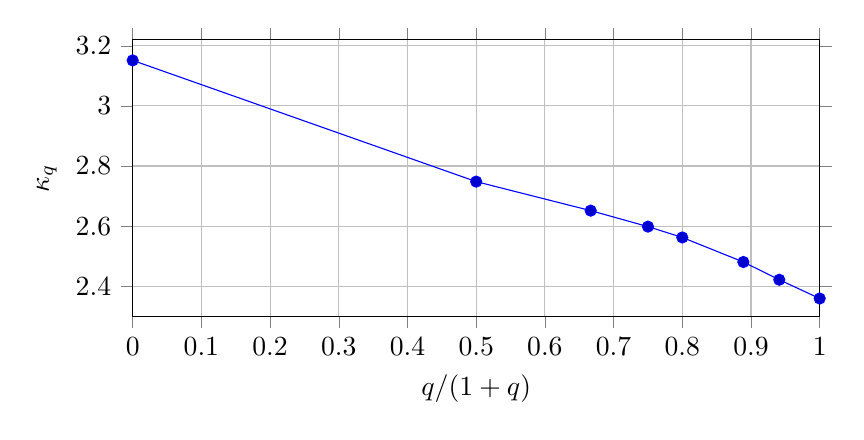
\begin{tikzpicture}
\begin{axis}[
 width=0.85\textwidth,
 height=0.42\textwidth,
 xlabel={$q/(1+q)$},
 ylabel={$\kappa_q$},
 xmin=0,xmax=1,
 ymin=2.30,ymax=3.22,
 grid=major,
 tick align=outside,
]
\addplot+[mark=*] coordinates {
 (0,3.1514961295)
 (0.5,2.7480700149)
 (0.6666666667,2.6514961295)
 (0.75,2.5983138062)
 (0.8,2.5622414703)
 (0.8888888889,2.4805809434)
 (0.9411764706,2.4214870020)
 (1,2.3590148791)
};
\end{axis}
\end{tikzpicture}
\end{center}

The monotone curve is not a cosmetic refinement: choosing one row answers one specific
notion of ``amplitude.''  Moving from $q=0$ to $q=\infty$ changes the power of $x$ by almost
$0.8$, an effect much larger than any logarithmic correction.

\section{Correction of the working draft}
\label{sec:draft-correction}

We can now state precisely which assertions in \cite{decay-draft} survive and which do not.

\subsection{Correct common feature}

The factor
\[
 \exp\!\left(-\frac{(\log x)^2}{2\log2}\right)
\]
is the common leading shell scale for every fixed finite $q$ and for the sharp shell
supremum.  It comes from the deterministic denominator
$2^{n(n+1)/2}$ in \eqref{eq:exact-factorization}.  This establishes rigorously the
``log-normal-like'' character of the largest and averaged values.

\subsection{The power $\log_2(2\pi)$ has a precise meaning}

The draft's power
\[
 x^{-\log(2\pi)/\log2}
\]
is exactly the RMS power, by \eqref{eq:kappa2}.  If the intended amplitude was the average
of $\AbsoluteValue{\Phiup}$, it must be replaced by $x^{-\kappa_1}$ with
$\kappa_1=2.748070014\ldots$.  If the intended object was the sharp global upper envelope,
it must be replaced by $x^{-\kappa_\infty}$ with
$\kappa_\infty=2.359014879\ldots$.  If the intended object was a typical fixed dyadic
phase, the power is $x^{-\kappa_0}$ with
$\kappa_0=3.151496129\ldots$.

\subsection{There is no global equivalent}

A statement of the form
\[
 \AbsoluteValue{\Phiup(x)}\sim C(\log x)^{-p}x^{-\kappa}
 \exp\!\left(-\frac{(\log x)^2}{2\log2}\right)
\]
cannot hold globally, for any $C>0,p,\kappa$, because $\Phiup$ vanishes at every integer.
It also cannot be repaired by replacing $\AbsoluteValue{\Phiup(x)}$ with the sequence of local maxima:
\Cref{cor:extrema-limsup-liminf} gives a positive limsup and zero liminf at the sharp upper
scale, while \Cref{thm:dyadic-valleys} exhibits a subsequence with a different leading
quadratic coefficient.

\subsection{No universal half-logarithm correction}

The term $-\tfrac12\log\log x$ asserted in the draft does not arise in any of the exact
shell normalizations above.  At the RMS scale, Parseval gives a pure exponential-in-$n$
identity.  At the arithmetic-mean scale, the transfer operator gives a simple Perron
eigenvalue and a positive constant.  At the uniform scale, the period-two orbit gives an
exact constant ratio.  Multiplication by $(\log x)^p$ destroys these normalizations unless
$p=0$.

A power of $n$ does occur in the exceptional valley asymptotic
\eqref{eq:valley-amplitude}, but its exponent is the integer zero multiplicity
$d=1+\TwoAdicValuation(r+1)$ and it accompanies the much faster factor $(b/N)^n$.  It is not a universal
correction to the generic shell envelope.

\section{Conclusions and further directions}
\label{sec:conclusion}

The Fourier transform of Rvachev's up-function has an unusually clean deterministic core
and an unusually rich oscillatory numerator.  The deterministic core is the log-square
factor
\[
 \exp\!\left(-\frac{(\log x)^2}{2\log2}\right),
\]
while the numerator is the modulus of a normalized Thue--Morse polynomial.  Once the two
are separated by \eqref{eq:master-normalization}, the apparently conflicting numerical
observations become compatible:

\begin{itemize}
\item typical values decay with power $\kappa_0=3.151496129\ldots$;
\item arithmetic means decay with power $\kappa_1=2.748070014\ldots$;
\item quadratic means decay with the draft's power
      $\kappa_2=\log_2(2\pi)=2.651496129\ldots$;
\item the largest values decay with the slower sharp power
      $\kappa_\infty=2.359014879\ldots$;
\item extrema near dyadic boundaries can decay with the stronger leading exponent
      $-(\log x)^2/\log2$.
\end{itemize}

Thus the phrase ``the exact decay rate'' must always be accompanied by a norm, an averaging
operation, or a specified subsequence.  For the original weak Cesaro criterion, the sharp
answer is $E_{\kappa_1}$, up to a constant.  For the sharp global upper envelope, the exact
answer is $E_{\kappa_\infty}$.  For the local-extremum sequence, there is no two-sided envelope on the common
log-normal--power scale: binary dynamics creates both period-two peaks and dyadic valleys.

Several natural continuations remain.  The pressure function $q\mapsto\log\rho_q$ gives a
multifractal large-deviation spectrum for fixed-phase values.  A parallel transfer formalism
on dyadic cylinders should describe the statistical distribution of the unit-interval
maxima $M_m$, not merely their global limsup and the explicit valley subsequences proved
here.  Both developments are well suited to eventual formalization because their analytic
input is concentrated in one explicit positive operator and a small collection of exact
renormalization identities.

\appendix

\section{Exact Collatz--Wielandt certificate for $\rho_1$}
\label{app:certificate}

The following SymPy script uses only exact rational arithmetic.  It constructs the rational
function in the proof of \Cref{prop:rho1-rigorous-bound}; Sturm's theorem, invoked by
\texttt{count\_roots}, certifies that the relevant numerators and denominators have no roots
on $[0,1]$.  Positivity at $t=0$ therefore proves positivity throughout the interval.

\begin{lstlisting}[style=code,language=Python]
import sympy as sp

t = sp.symbols("t", real=True)
u = 2*t/(1+t**2)
v = (1-t**2)/(1+t**2)

c = sp.Rational(376189, 10**6)
d = sp.Rational(-69093, 10**6)
e = sp.Rational(15483, 10**6)
F = lambda z: 1 + c*z + d*z**2 + e*z**3

R = sp.cancel((u*F(u) + v*F(v)) / (2*F(2*u*v)))
lo = sp.Rational(66126807, 10**8)
hi = sp.Rational(66134891, 10**8)

for expr in (R - lo, hi - R):
    num, den = map(lambda p: sp.Poly(p, t),
                   sp.together(expr).as_numer_denom())
    assert num.eval(0) > 0 and den.eval(0) > 0
    assert num.count_roots(0, 1) == 0
    assert den.count_roots(0, 1) == 0

print("Certified:", lo, "< rho_1 <", hi)
\end{lstlisting}

For the high-precision decimal, one may replace the exact certificate by a Chebyshev
collocation matrix.  The rapid stabilization displayed in \Cref{sec:numerics} is typical
for this analytic weighted-composition operator.

\section{Notation cross-reference}
\label{app:notation}

\begin{center}
\begin{tabularx}{\textwidth}{@{}lX@{}}
\toprule
Symbol & Meaning\\
\midrule
$\Phiup=\widehat{\RvachevUp}$ & Fourier transform of Rvachev's up-function\\
$a$ & $\log2$\\
$T$ & doubling map $x\mapsto2x\pmod1$\\
$s(x)$ & $\AbsoluteValue{\sin(\pi x)}$\\
$B_n(y)$ & $\prod_{j=1}^n s(T^jy)$\\
$E_\kappa(x)$ & $x^{-\kappa}\exp(- (\log x)^2/(2\log2))$\\
$W_\kappa(y)$ & bounded dyadic phase factor in \eqref{eq:master-normalization}\\
$\mathcal L_q$ & weighted Perron operator \eqref{eq:transfer-operator}\\
$\rho_q$ & Perron root of $\mathcal L_q$\\
$\Lambda_q$ & $\rho_q^{1/q}$, the $L^q$ numerator growth per dyadic level\\
$\kappa_q$ & sharp power in the normalized $L^q$ shell decay\\
$M_m$ & unique maximum of $\AbsoluteValue{\Phiup}$ on $[m,m+1]$\\
\bottomrule
\end{tabularx}
\end{center}

\begin{thebibliography}{99}

\bibitem{arias1982}
J. Arias de Reyna,
\emph{An infinitely differentiable function with compact support: Definition and properties},
English translation of \emph{Definici\'on y estudio de una funci\'on indefinidamente
diferenciable de soporte compacto}, Rev. Real Acad. Cienc. Exact. F\'is. Natur. Madrid
\textbf{76} (1982), 21--38; arXiv:1702.05442 (2017).

\bibitem{arias2018}
J. Arias de Reyna,
\emph{Arithmetic of the Fabius function},
Integers \textbf{18} (2018), Paper A51; arXiv:1702.06487.

\bibitem{baladi}
V. Baladi,
\emph{Positive Transfer Operators and Decay of Correlations},
Advanced Series in Nonlinear Dynamics, vol.~16, World Scientific, 2000.

\bibitem{fabius}
J. Fabius,
\emph{A probabilistic example of a nowhere analytic $C^\infty$-function},
Z. Wahrscheinlichkeitstheorie verw. Gebiete \textbf{5} (1966), 173--174,
\href{https://doi.org/10.1007/BF00536652}{doi:10.1007/BF00536652}.

\bibitem{fan1997}
A.-H. Fan,
\emph{Multifractal analysis of infinite products},
J. Statist. Phys. \textbf{86} (1997), 1313--1336,
\href{https://doi.org/10.1007/BF02183625}{doi:10.1007/BF02183625}.

\bibitem{fan-schmeling-shen}
A. Fan, J. Schmeling, and W. Shen,
\emph{$L^\infty$-estimation of generalized Thue--Morse trigonometric polynomials and
ergodic maximization},
Discrete Contin. Dyn. Syst. \textbf{41} (2021), 297--327,
\href{https://doi.org/10.3934/dcds.2020363}{doi:10.3934/dcds.2020363}.

\bibitem{gelfond}
A. O. Gel'fond,
\emph{Sur les nombres qui ont des propri\'et\'es additives et multiplicatives donn\'ees},
Acta Arith. \textbf{13} (1967/68), 259--265,
\href{https://doi.org/10.4064/aa-13-3-259-265}{doi:10.4064/aa-13-3-259-265}.

\bibitem{jessen-wintner}
B. Jessen and A. Wintner,
\emph{Distribution functions and the Riemann zeta function},
Trans. Amer. Math. Soc. \textbf{38} (1935), 48--88.

\bibitem{mse-extrema}
V. Reshetnikov,
\emph{Extrema of an infinite product of sinc functions},
Mathematics Stack Exchange, question 2742261 (2018),
\url{https://math.stackexchange.com/questions/2742261/}.

\bibitem{mse-decay}
V. Reshetnikov,
\emph{Asymptotic decay rate of an infinite product of sinc functions},
Mathematics Stack Exchange, question 2745497 (2018),
\url{https://math.stackexchange.com/questions/2745497/}.

\bibitem{proveit}
V. Reshetnikov,
\emph{ProveIt: Analysis/FabiusFunction}, GitHub repository,
\url{https://github.com/VladimirReshetnikov/ProveIt/tree/main/Analysis/FabiusFunction}.

\bibitem{decay-draft}
V. Reshetnikov,
\emph{Decay rate conjecture}, working draft in the \texttt{ProveIt} repository,
\url{https://github.com/VladimirReshetnikov/ProveIt/blob/main/Analysis/FabiusFunction/docs/semi-formalized-research-frontiers/drafts/Decay%20rate%20conjecture/Decay%20rate%20conjecture.tex}.

\bibitem{queffelec}
M. Queff\'elec,
\emph{Questions around the Thue--Morse sequence},
Unif. Distrib. Theory \textbf{13} (2018), no.~1, 1--25,
\href{https://doi.org/10.1515/udt-2018-0001}{doi:10.1515/udt-2018-0001}.

\bibitem{rvachev1971}
V. L. Rvachev and V. A. Rvachev,
\emph{On one compactly supported function},
Dokl. Akad. Nauk Ukrainian SSR, Ser.~A, no.~8 (1971), 705--707
(in Ukrainian).

\end{thebibliography}

\end{document}
